\documentclass[a4paper]{article}
\usepackage{multicol}
\usepackage[utf8]{inputenc}
\usepackage[margin=1.2cm]{geometry}
\usepackage{graphicx}
\renewcommand{\familydefault}{phv}

\begin{document}
\begin{multicols}{3}
  \section{Wärmelehre}
  $ 0 K = - 273.15 C^\circ $ (allgemein $ 0 K = 273^\circ C $)
  
  \section{Wärmeausdehnung}
  \subsection{Linear}
  
  $ \Delta l = \alpha * l_0 * \Delta \vartheta $ also
  
  $ l = l_0 * (1 + \alpha * \Delta \vartheta) $
  
  $ \alpha = \frac{\Delta l}{l_0 * \Delta \vartheta} $
  
  \subsection{Volumen}
  
  \textbf{Initialzustand:}\\
  
  $ V_0 = l_0 * b_0 * h_0 $
  
  \textit{In erwärmten Zustand}\\
  
  $ V = l * b * h = l_0 (1 + \alpha * \Delta \vartheta) * b_0 (1 + \alpha * \Delta \vartheta) * h_0 (1 + \alpha * \Delta \vartheta) $\\
  
  \textbf{Vereinfacht:}\\
  
  $ V \approx V_0 (1 + 3 * \alpha * \Delta \vartheta) $\\
  
  $ \gamma = 3 * \alpha $ \\
  
  \textit{Volumenzunahme $\Delta V$:}\\
  $ \Delta V = V_0 * \gamma  * \Delta \vartheta $ \\
  
  \section{Wärmeenergie}
  
  \textbf{Wärmeenergie}: $[Q] = Joule (J) = Newtonmeter (Nm)$\\
  \textbf{Wärmekapazität}: $ [c] = \frac{kJ}{kg K}$\\
  
  \textbf{Beispiele für $ c $}\\ 
  \begin{tabular}{ll}
  	Wasser & 4.19 \\
  	Alkohol & 2.43 \\
  	Wasserstoff & 14.3
  \end{tabular}\\
  
  \textbf{Berechnung:}\\
  $ \Delta Q = c * m * \Delta \vartheta $
  
  \subsection{Wärmeinhalt}
  $ Q = m * c * \vartheta $
  \subsection{Wärmekapazität $[C]$}
  
  $ [C] = \frac{J}{K} $
  
  \textbf{Berechnung}\\
  $ C = \frac{\Delta Q}{\Delta \vartheta} $\\
  
  Oder \\
  
  $ C = m * c $
  
  \subsection{Wärmemischung}
  
  $ |\Delta Q_{ab}| = | \Delta Q_{auf} | $\\
  oder\\
  $c_1 * m_1  * (\vartheta_1 - \vartheta_m) = c_2 * m_2 * (\vartheta_m - \vartheta_2) $\\
  (Wenn abs wert, ist reihenfolge v. $ \vartheta_{1,2}$ und $ \vartheta_m $ egal)
  
  \subsection{Verbrennungsenergie}
  
  \textit{Heizwert}: $ H = \frac{Q}{m}; [H] = \frac{J}{kg} $
  \section{Aggregatszustände}
  
  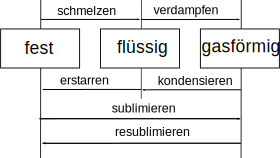
\includegraphics[width=2in]{agregat}
  
  \subsection{Schmelzwärme}
  
  $ L_F = \frac{Q_s}{m} $
  
  \subsection{Verdampfungswärme}
  
  $ Q_v = \frac{Q_v}{m} $
\end{multicols}

%\begin{table}
%	\begin{tabular}{|lr}|lr|lr|}
		%Aluminium & $ 24 * 10^{-6} $ & Gusseisen & $10 * 10^{-6} $ & Platin & $ 9 * 10^{-6} $ \\
		%Blei & $ 29 * 10^{-6} $ & Holz parallel zu Faser & $ 3 .. 6 * 10^{-6} $ & Polyvonychlorid  & $ %8 * 10^{-6} $ \\
		%Celluloid 100 * 10^-6 Holz querz zur Faster 0.2 .. 0.6 * 10^-6 Porzelan 5 * 10^-6
		%Elektron 24 * 10^-6 Invar 1.6 * 10^-6 Quarzglas
	%\end{tabular}
	%\caption{Mittlere Längeausdehnungskoeffizienten zwischen $ 0^{\circ}C $ und $ 100^{\circ}C $ in $ K^{-1} $ von festen Stoffen}
%\end{table}

\end{document}
